% =====================================================================
\newpage
\part{Modelos de Segundo Parcial}
% =====================================================================
\section{Modelo A}

\subsection{Ejercicio 1 --- Cajas registradoras}
\begin{enun}
Hay 3 cajas. Dos clientes eligen cada uno una caja al azar, en forma independiente. $X$ = número de clientes que eligen la caja 1; $Y$ = número que eligen la caja 2.
a) Tabla conjunta. \ b) ¿Independientes? \ c) ¿Misma distribución? \ d) $\Cov(X,Y)$.
\end{enun}
\begin{metodo}
Cada cliente elige caja 1, 2 o 3 con probabilidad $\frac13$ cada una, de forma independiente. Hay $3^2=9$ resultados equiprobables, cada uno con probabilidad $\frac19$, y se cuenta cuántos dan cada par $(x,y)$. Es una distribución trinomial (multinomial) con $n=2$.
\end{metodo}
\inciso{a) Tabla conjunta}
Resultados (caja del cliente 1, caja del cliente 2):
(1,1): $x=2,y=0$; \ (2,2): $x=0,y=2$; \ (3,3): $x=0,y=0$; \ (1,2),(2,1): $x=1,y=1$; \ (1,3),(3,1): $x=1,y=0$; \ (2,3),(3,2): $x=0,y=1$.
\begin{center}
\renewcommand{\arraystretch}{1.3}
\begin{tabular}{@{}c|ccc|c@{}}
\toprule
$p(x,y)$ & $y=0$ & $y=1$ & $y=2$ & $p_X(x)$\\\midrule
$x=0$ & $1/9$ & $2/9$ & $1/9$ & $\mathbf{4/9}$\\
$x=1$ & $2/9$ & $2/9$ & $0$ & $\mathbf{4/9}$\\
$x=2$ & $1/9$ & $0$ & $0$ & $\mathbf{1/9}$\\\midrule
$p_Y(y)$ & $\mathbf{4/9}$ & $\mathbf{4/9}$ & $\mathbf{1/9}$ & 1\\\bottomrule
\end{tabular}
\end{center}
\inciso{b) Independencia}
$p(2,2)=0$, pero $p_X(2)\,p_Y(2)=\frac19\cdot\frac19=\frac1{81}\neq0$. \textbf{No son independientes}: hay solo dos clientes, así que si los dos van a la caja 1, ninguno va a la caja 2.

\inciso{c) ¿Misma distribución?}
\textbf{Sí}: las dos marginales son $(4/9;\,4/9;\,1/9)$, es decir, $X\sim Y\sim\mathrm{Bin}(2;\,1/3)$. Tienen la misma distribución, pero no son la misma variable ni son independientes.

\inciso{d) Covarianza}
$\E(X)=\E(Y)=2\cdot\frac13=\frac23$. \quad $\E(XY)$: solo aporta la celda $(1,1)$: $\E(XY)=1\cdot1\cdot\frac29=\frac29$.
\[
\Cov(X,Y)=\frac29-\frac23\cdot\frac23=\frac29-\frac49=\res{-\frac29=-0{,}2222}
\]
(Coincide con la fórmula de la multinomial, $\Cov=-n\,p_1p_2=-2\cdot\frac13\cdot\frac13$.)

\subsection{Ejercicio 2 --- Tamaño de muestra para una proporción}
\begin{enun}
¿Cuántos clientes hay que encuestar para que la fracción muestral de insatisfechos se desvíe a lo sumo 0,15 de la poblacional, con probabilidad no menor a 0,98? Definir variables, distribución y parámetros; justificar con propiedades y teoremas.
\end{enun}
\begin{metodo}
$X_i=1$ si el cliente $i$ está insatisfecho y 0 si no: $X_i\sim$ Bernoulli$(p)$, independientes.
$T=\sum X_i\sim\mathrm{Bin}(n;p)$ y $\hat P=T/n$, con $\E(\hat P)=p$ y $\V(\hat P)=p(1-p)/n$ (propiedades de la esperanza y la varianza).
Por el \textbf{TCL}, para $n$ grande, $\hat P\approx\Nor\big(p;\,p(1-p)/n\big)$. Como $p$ es desconocido, se usa el peor caso $p(1-p)\le\frac14$.
\end{metodo}
\paso{Planteo.}
\[
P\big(|\hat P-p|\le0{,}15\big)\ge0{,}98\iff P\Big(|Z|\le\frac{0{,}15}{\sqrt{p(1-p)/n}}\Big)\ge0{,}98\iff\frac{0{,}15\sqrt n}{\sqrt{p(1-p)}}\ge z_{0,01}=2{,}3263.
\]
\paso{Despeje.} $n\ge\dfrac{z_{0,01}^2\,p(1-p)}{0{,}15^2}$. Como $p$ es desconocido, se toma el peor caso $p(1-p)=\frac14$, que vale para cualquier $p$:
\[
n\ge\frac{2{,}3263^2\cdot0{,}25}{0{,}0225}=60{,}13\ \Rightarrow\ \res{n=61}
\]
\begin{resp}
Hay que encuestar \textbf{61 clientes}. Con ese $n$ se cumple para cualquier valor de $p$.
Si se usara la desigualdad de Chebyshev, que no requiere aproximación normal, se obtendría $P(|\hat P-p|>0{,}15)\le\frac{1}{4n(0{,}15)^2}\le0{,}02$, de donde $n\ge556$: más conservador.
\end{resp}

\subsection{Ejercicio 3 --- Redacción de la conclusión}
\begin{enun}
$H_0$: el método no es efectivo. $H_1$: el método es efectivo. Si se \emph{rechaza} $H_0$, ¿está bien la conclusión ``No hay evidencia significativa para concluir que el método no es efectivo''?
\end{enun}
\begin{resp}
\textbf{No está bien expresada.} Rechazar $H_0$ significa que los datos aportan evidencia significativa \emph{a favor de $H_1$}. La frase dada habla de ``falta de evidencia'', que es el lenguaje de \emph{no rechazar}, y además se refiere a la afirmación de $H_0$ en vez de a la de $H_1$.
\textbf{Corrección:} ``Hay evidencia significativa (al nivel $\alpha$) para concluir que el método \emph{es} efectivo.''
\end{resp}

\subsection{Ejercicio 4 --- Nivel de significación y error tipo II}
\begin{enun}
$\sigma=8{,}4$; $H_0:\mu=80$ vs.\ $H_1:\mu<80$; $n=100$. Se rechaza $H_0$ si $\xb\le78{,}2$.
a) Nivel de significación. \ b) Error tipo II en contexto y su probabilidad si $\mu$ difiere de 80 en 1,3. \ c) Conclusión si el valor $P$ es 0,011.
\end{enun}
\begin{metodo}
Con $n=100$, por el TCL $\Xb\approx\Nor(\mu;\,\sigma^2/n)$, con $\sigma/\sqrt n=8{,}4/10=0{,}84$. $\alpha$ y $\beta$ se calculan como áreas bajo esa normal, usando la región de rechazo dada.
\end{metodo}
\inciso{a) Nivel de significación}
\[
\alpha=P(\Xb\le78{,}2\,|\,\mu=80)=\Phi\Big(\frac{78{,}2-80}{0{,}84}\Big)=\Phi(-2{,}1429)=\res{0{,}0161}
\]
\inciso{b) Error tipo II}
\textbf{Significado:} no rechazar $H_0$ (concluir que la media es 80) cuando en realidad es menor.
Como $H_1$ es $\mu<80$, ``difiere en 1,3'' significa $\mu=80-1{,}3=78{,}7$:
\[
\beta=P(\Xb>78{,}2\,|\,\mu=78{,}7)=1-\Phi\Big(\frac{78{,}2-78{,}7}{0{,}84}\Big)=1-\Phi(-0{,}5952)=\res{0{,}7242}
\]
Esta prueba tiene poca potencia (0,2758) para detectar una diferencia de 1,3.

\inciso{c) Valor $P=0{,}011$}
Se rechaza $H_0$ si $P\le\alpha$. Con el nivel de esta prueba, $\alpha=0{,}0161$, se tiene $0{,}011<0{,}0161$: \textbf{se rechaza $H_0$}. Hay evidencia de que $\mu<80$. (Con $\alpha=0{,}05$ también se rechazaría; con $\alpha=0{,}01$, no.)

\subsection{Ejercicio 5 --- Verdadero o falso}
\inciso{a) VERDADERA}
$Y=a\Xb_1+(1-a)\Xb_2$ con $n_2=4n_1$. Por linealidad, y porque $\E(\Xb_i)=\mu$:
\[
\E(Y)=a\mu+(1-a)\mu=\mu\quad\Rightarrow\ \text{insesgado para todo }a.
\]
Las muestras son independientes, así que
\[
\V(Y)=a^2\frac{\sigma^2}{n_1}+(1-a)^2\frac{\sigma^2}{4n_1}=\frac{\sigma^2}{n_1}\Big[a^2+\frac{(1-a)^2}{4}\Big].
\]
Se minimiza derivando: $\frac{d}{da}\big[a^2+\frac{(1-a)^2}4\big]=2a-\frac{(1-a)}{2}=0\Rightarrow4a=1-a\Rightarrow\res{a=\frac15}$. La derivada segunda es $2+\frac12>0$, así que es un mínimo.
(Es el promedio ponderado por los tamaños: $a=\frac{n_1}{n_1+n_2}=\frac15$.)

\inciso{b) VERDADERA}
La longitud del IC con $\sigma$ conocido es $L=2z_{\alpha/2}\sigma/\sqrt n$. Para tener $L'=L/2$ con la misma confianza: $\frac{1}{\sqrt{n'}}=\frac{1}{2\sqrt n}\Rightarrow\sqrt{n'}=2\sqrt n\Rightarrow n'=4n$. Hay que \textbf{cuadruplicar} $n$.

\inciso{c) FALSA}
La población es normal, $\sigma$ es desconocido y $n=9$ es chico, así que corresponde $t$ con 8 g.l.: $t_{0,015;\,8}=2{,}6338$.
\[
6\pm2{,}6338\cdot\frac{0{,}12}{\sqrt9}=6\pm0{,}1054\ \Rightarrow\ \res{(5{,}8946;\ 6{,}1054)}
\]
El intervalo del enunciado, $(5{,}9132;\,6{,}0868)$, tiene semiamplitud $0{,}0868=2{,}1701\cdot0{,}04$: se calculó con $z_{0,015}=2{,}1701$, que no corresponde porque $\sigma$ es desconocido. Por eso la afirmación es \textbf{falsa}.

% =====================================================================
\newpage
\section{Modelo B}

\subsection{Problema 1 --- Circuito de tres componentes}
\begin{enun}
A y B en serie, y esa rama en paralelo con C. Los componentes son independientes y cada uno funciona con probabilidad 0,92. $X$ = cantidad de componentes que funcionan; $Y=1$ si el circuito funciona y $0$ si no.
a) $p_{XY}(x,y)$. \ b) Si funciona a lo sumo un componente, probabilidad de que el circuito no funcione. \ c) Coeficiente de correlación. \ d) De 100 circuitos, probabilidad de que funcionen al menos 96.
\end{enun}
\begin{metodo}
El circuito funciona si y solo si $(A\cap B)\cup C$. Se recorren los $2^3=8$ estados (independencia: producto de probabilidades, con $q=0{,}92$ y $1-q=0{,}08$) y se anota $(x,y)$. Además, $X\sim\mathrm{Bin}(3;\,0{,}92)$.
\end{metodo}
\inciso{a) Función de probabilidad conjunta}
\begin{center}
\renewcommand{\arraystretch}{1.25}
\begin{tabular}{@{}lccc@{}}
\toprule
Estado (funcionan) & Probabilidad & $x$ & $y$\\\midrule
ninguno & $0{,}08^3=0{,}000512$ & 0 & 0\\
solo A, o solo B & $2\cdot0{,}92\cdot0{,}08^2=0{,}011776$ & 1 & 0\\
solo C & $0{,}92\cdot0{,}08^2=0{,}005888$ & 1 & 1\\
AB, AC o BC & $3\cdot0{,}92^2\cdot0{,}08=0{,}203136$ & 2 & 1\\
ABC & $0{,}92^3=0{,}778688$ & 3 & 1\\\bottomrule
\end{tabular}
\qquad
\begin{tabular}{@{}c|cc|c@{}}
\toprule
$p$ & $y=0$ & $y=1$ & $p_X$\\\midrule
$x=0$ & 0,000512 & 0 & 0,000512\\
$x=1$ & 0,011776 & 0,005888 & 0,017664\\
$x=2$ & 0 & 0,203136 & 0,203136\\
$x=3$ & 0 & 0,778688 & 0,778688\\\midrule
$p_Y$ & 0,012288 & 0,987712 & 1\\\bottomrule
\end{tabular}
\end{center}
Con dos componentes funcionando, el circuito siempre funciona: si son A y B, por la rama en serie; si uno de los dos es C, por C.

\inciso{b) $P(Y=0\,|\,X\le1)$}
\[
P(Y=0\,|\,X\le1)=\frac{p(0,0)+p(1,0)}{p_X(0)+p_X(1)}=\frac{0{,}000512+0{,}011776}{0{,}000512+0{,}017664}=\frac{0{,}012288}{0{,}018176}=\res{0{,}6761}
\]
\inciso{c) Coeficiente de correlación}
$\E(X)=3(0{,}92)=2{,}76$; $\V(X)=3(0{,}92)(0{,}08)=0{,}2208$.
$\E(Y)=0{,}987712$; $\V(Y)=0{,}987712\cdot0{,}012288=0{,}012137$.
$\E(XY)=1(0{,}005888)+2(0{,}203136)+3(0{,}778688)=2{,}748224$.
\[
\Cov=2{,}748224-2{,}76\cdot0{,}987712=0{,}022139;\qquad
\rho=\frac{0{,}022139}{\sqrt{0{,}2208\cdot0{,}012137}}=\res{0{,}4277}
\]
\textbf{Interpretación:} hay una asociación lineal positiva y moderada. Cuantos más componentes funcionan, más probable es que funcione el circuito. No es una relación lineal fuerte porque $Y$ solo toma 0 o 1, y vale 1 casi siempre.

\inciso{d) Al menos 96 de 100 circuitos funcionan}
Sea $W$ = número de circuitos que funcionan, $W\sim\mathrm{Bin}(100;\,0{,}987712)$. Hay pocos fallos esperados: $n(1-p)=1{,}2288<5$, así que la aproximación normal \textbf{no} es adecuada. Se usa la de \textbf{Poisson} para la cantidad de fallas $F=100-W\approx\mathrm{Poisson}(\lambda=1{,}2288)$:
\[
P(W\ge96)=P(F\le4)=\sum_{k=0}^{4}e^{-1{,}2288}\frac{1{,}2288^k}{k!}=\res{0{,}9915}
\]
(El valor binomial exacto es 0,9920. La normal con corrección por continuidad daría 0,9985, que es peor.)

\subsection{Problema 2 --- Estimador insesgado de $a^2$}
\begin{enun}
$X_1,\dots,X_n$ m.a.\ de $X\sim U(-a;\,a)$. Demostrar que $T=\frac3n\sum X_i^2$ es un estimador insesgado de $a^2$.
\end{enun}
\begin{metodo}
Se usan la linealidad de la esperanza y que $\E(X^2)=\V(X)+\E(X)^2$, con $\V=\frac{(b-a)^2}{12}$ para la uniforme.
\end{metodo}
\paso{Paso 1.} Para $X\sim U(-a;a)$: $\E(X)=0$ y $\V(X)=\frac{(2a)^2}{12}=\frac{a^2}{3}$, así que $\E(X_i^2)=\frac{a^2}{3}$.

\paso{Paso 2.}
\[
\E(T)=\frac3n\sum_{i=1}^n\E(X_i^2)=\frac3n\cdot n\cdot\frac{a^2}{3}=a^2.\qquad\blacksquare
\]
Como $\E(T)=a^2$ para todo $a$, $T$ es \textbf{insesgado} para $a^2$.

\subsection{Problema 3 --- Distancia de frenado}
\begin{enun}
$n=20$ pruebas, $\xb=109{,}8$ m, $s=20$ m. a) IC de nivel 0,90 para $\mu$; ¿qué información falta? b) Si $\mu=110$, ¿el gráfico de 100 intervalos corresponde a un nivel de 0,95?
\end{enun}
\inciso{a) IC 90\,\%}
\textbf{Información omitida:} que la distancia de frenado tiene distribución \textbf{normal}. Con $\sigma$ desconocido y $n=20<30$, esa suposición es la que permite usar $T=\frac{\Xb-\mu}{S/\sqrt n}\sim t_{19}$.
\[
t_{0,05;19}=1{,}7291;\qquad109{,}8\pm1{,}7291\cdot\frac{20}{\sqrt{20}}=109{,}8\pm7{,}7329\ \Rightarrow\ \res{102{,}07\le\mu\le117{,}53\ \text{m}}
\]
\inciso{b) ¿El gráfico corresponde a 95\,\%?}
\paso{Conteo.} En el gráfico hay \textbf{14 intervalos en rojo} (no contienen a la media) de 100: una cobertura del 86\,\%.

\paso{Comparación.} Con 95\,\% de confianza, la cantidad de intervalos que fallan es $F\sim\mathrm{Bin}(100;\,0{,}05)$, con media 5 y desvío 2,18. Ver 14 o más fallos tiene probabilidad $P(F\ge14)=0{,}0005$: es muy improbable.
\begin{resp}
\textbf{No corresponde} a un nivel de 0,95: con 95\,\% se esperan unos 5 intervalos fallidos, y hay 14 (86\,\% de cobertura). Además, la línea de referencia está en 109,39 y no en $\mu=110$: si el valor verdadero fuera 110, habría que contar los intervalos que no contienen a 110.
\end{resp}

\subsection{Problema 4 --- Vigas de magnesio}
\begin{enun}
La media del porcentaje de defectos no puede superar el 5\,\%. Si $\xb>5{,}5$ se detiene la producción, con probabilidad de equivocarse de 0,01. El porcentaje de defectos es normal con $\sigma^2=1$.
a) Hipótesis, estadístico, región y $n$. \ b) ¿El gráfico es una curva de potencia? \ c) Valor $P$ límite para no certificar.
\end{enun}
\inciso{a) Planteo y tamaño de muestra}
\[
H_0:\mu=5\ (\mu\le5)\qquad\text{vs.}\qquad H_1:\mu>5;\qquad Z=\frac{\Xb-5}{1/\sqrt n}\ \overset{H_0}{\sim}\ \Nor(0;1)
\]
(exacto, porque la población es normal y $\sigma$ es conocido). Región de rechazo: $\xb>5{,}5$, con $\alpha=P(\Xb>5{,}5\,|\,\mu=5)=0{,}01$.
\[
\frac{5{,}5-5}{1/\sqrt n}=z_{0,01}=2{,}3263\ \Rightarrow\ \sqrt n=4{,}6527\ \Rightarrow\ n=21{,}65\ \Rightarrow\ \res{n=22}
\]
Con $n=22$, la regla $\xb>5{,}5$ da $\alpha=0{,}0095\le0{,}01$ \checkmark. Dicho con el estadístico: se rechaza si $z_0>2{,}3263$.

\inciso{b) ¿Es una curva de potencia?}
La potencia es $\pi(\mu)=P(\Xb>5{,}5\,|\,\mu)$, que es \textbf{creciente} en $\mu$: $\pi(5)=0{,}0095$, $\pi(5{,}5)=0{,}5$, $\pi(6)=0{,}9905$.
El gráfico dado es \textbf{decreciente}: vale $\approx1$ en $\mu=5$ y $\approx0$ en $\mu=6$.
\begin{figure}[h]
\centering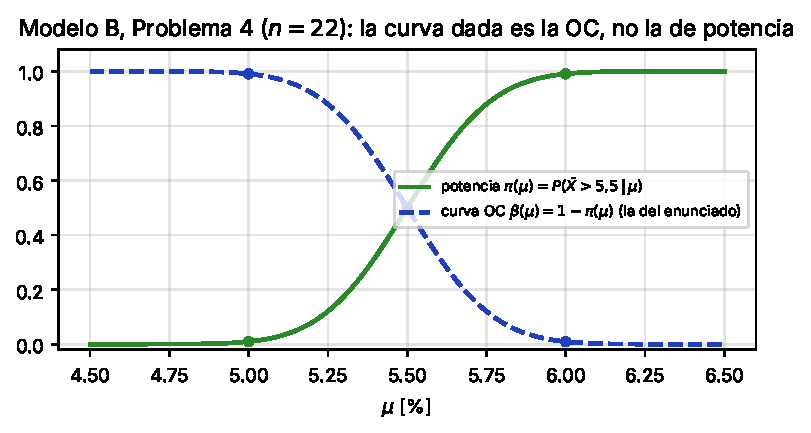
\includegraphics[width=0.78\textwidth]{fig/mbpot.pdf}
\end{figure}
\begin{resp}
\textbf{No}, es la curva \textbf{OC} $\beta(\mu)=1-\pi(\mu)$. Dos puntos lo muestran:
\begin{itemize}
\item En $\mu=5$ ($H_0$ cierta) el gráfico marca $\approx0{,}99=1-\alpha$, la probabilidad de \emph{no} rechazar. La potencia valdría $\alpha\approx0{,}01$.
\item En $\mu=6$ el gráfico marca $\approx0{,}01$, que es $\beta(6)$: la probabilidad de no detener la producción cuando la media es 6. La potencia valdría 0,99.
\end{itemize}
En $\mu=5{,}5$ las dos curvas valen 0,5.
\end{resp}

\inciso{c) Valor $P$ para no certificar}
No certificar equivale a rechazar $H_0$ (concluir que $\mu>5$), y eso ocurre si $P\le\alpha$. El valor $P$ debe ser como \textbf{máximo 0,01}: no se certifica si $P\le0{,}01$; con la regla exacta para $n=22$, $P\le0{,}0095$.
